\section{Geometrical acceptance}
A geometrical acceptance is calculated using a Monte Carlo technique.
Events are generated flat in the variables $W$, $Q^2$, $\cos\theta^*$, $\phi^*$, $\phi_e$,
then the following quantities are calculated (see App. \ref{sec:kinema} for the meaning 
of the quantities)
\begin{equation}
\begin{array}{c}
 \nu = q_0 = \Dfrac{W^2 + Q^2 - M_P^2}{2M_P} \Rightarrow E' = E - \nu\\ \\
 \cos\theta_{e'} = (1-\Dfrac{Q^2}{2EE'}) \\ \\ 
 p_{\pi^0}^* = p_P^* = \Dfrac{\sqrt{ ( W^2 - (M_P + M_{\pi^0})^2 )
                                     ( W^2 - (M_P - M_{\pi^0})^2 ) }}{2W}
\end{array}
\end{equation}
so that the proton four momentum in the c.m. $p_P^*$ and the electron four momentum in the lab $e_{\mu}'$ are obtained.
A Lorentz transformation from the resonance system to the lab system gives the proton four momentum in 
the lab $P'_{\mu}$. 

The $e_{\mu}'$ and $P'_{\mu}$ four vectors are then subjucted to the same cuts that make
use of four vector momenta applied to real data. These are the fiducial cuts 
(sections \ref{sec:fid_e} and  \ref{sec:fid_p}) 
and the B.H. cuts (section \ref{sec:bethe}). The acceptance $A$ is calculated for each bin.

\begin{equation}
 A = A(W, Q^2, \cos\theta^*, \phi^*) = \Dfrac{\# \,\,accepted \,\,events}
                                             {\# \,\, generated  \,\, events}\,\,(W, Q^2, \cos\theta^*, \phi^*)
\end{equation}					     

This method is convenient because it is very fast: billions of events can be processed in only a few hours.
However it does not take into account
the detector response. For example effects like bin migration, multiple scattering, finite
momentum resolution, do not enter in this model. Yet, the geometrical acceptance can
be a good approximation for a real acceptance calculation.
\F{fig:geom_acctp} show an example of the acceptance distribution as a function of $\cos\theta^*$ and $\phi^*$. 

\begin{figure}[h]
 \begin{center}
 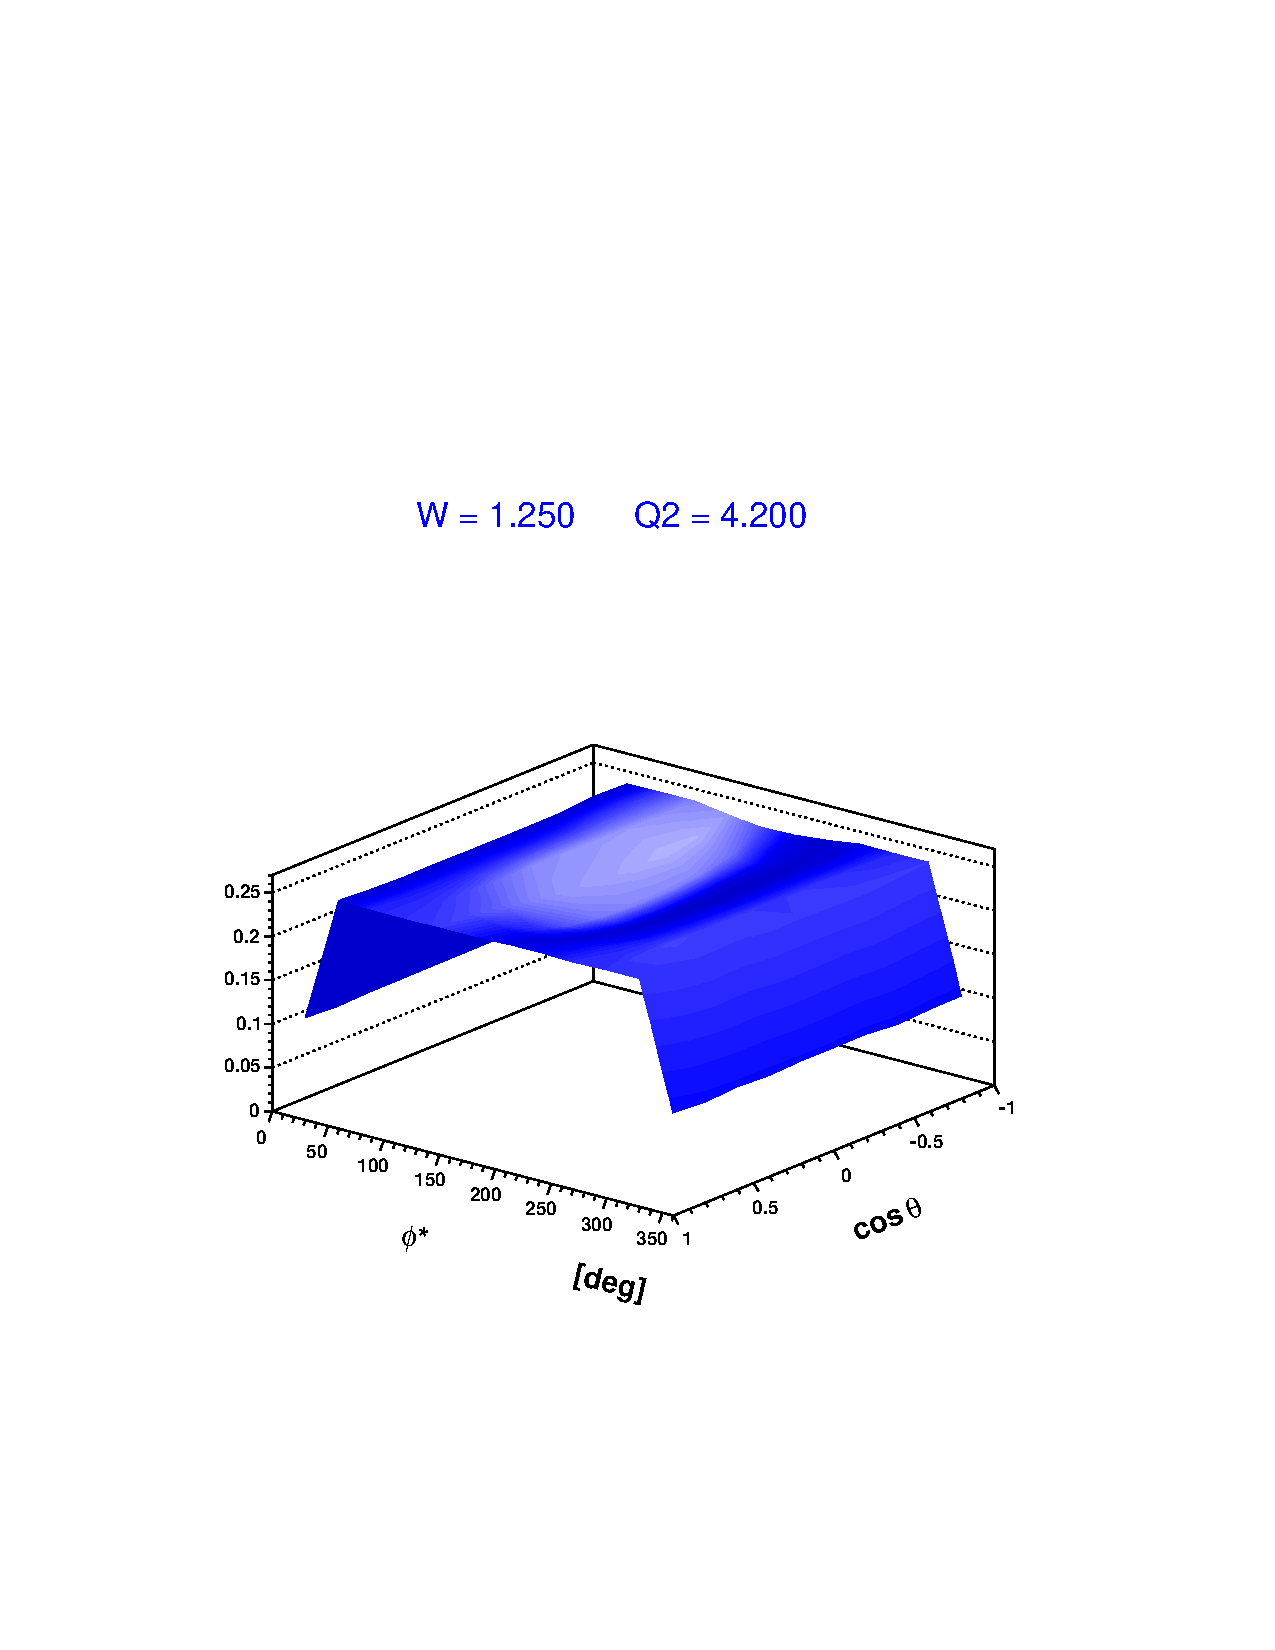
\includegraphics[width = 12cm, bb=80 120 500 600]{acceptance/img/geom_acc_tp} 
  \caption[Geometrical acceptance for $W = 1.25 \pm 0.01$ GeV and  $Q^2$ from $3.79$ to $4.52$ GeV$^2$
                     as a function of $\cos\theta^*$ and $\phi^*$]
          { Geometrical acceptance for $1.24 \le W \le 1.26$ GeV and  $Q^2$ 
	             from $3.79$ to $4.52$ GeV$^2$
                     as a function of the $\pi^0$ angles in the c.m. frame 
		     $\cos\theta^*$ and $\phi^*$. The B.H. cut affects
		     the distributions at $\phi_{\pi^0}^*$ extremes ($0^0$ and $360^0$) 
		     because it cuts out events 
		     with $\phi_P^* \sim 180^0$ (the pions and the proton have opposite momentum 
		     in the c.m.).}
 \label{fig:geom_acctp}
 \end{center}
\end{figure}


% \begin{figure}[h]
%  \begin{center}
%  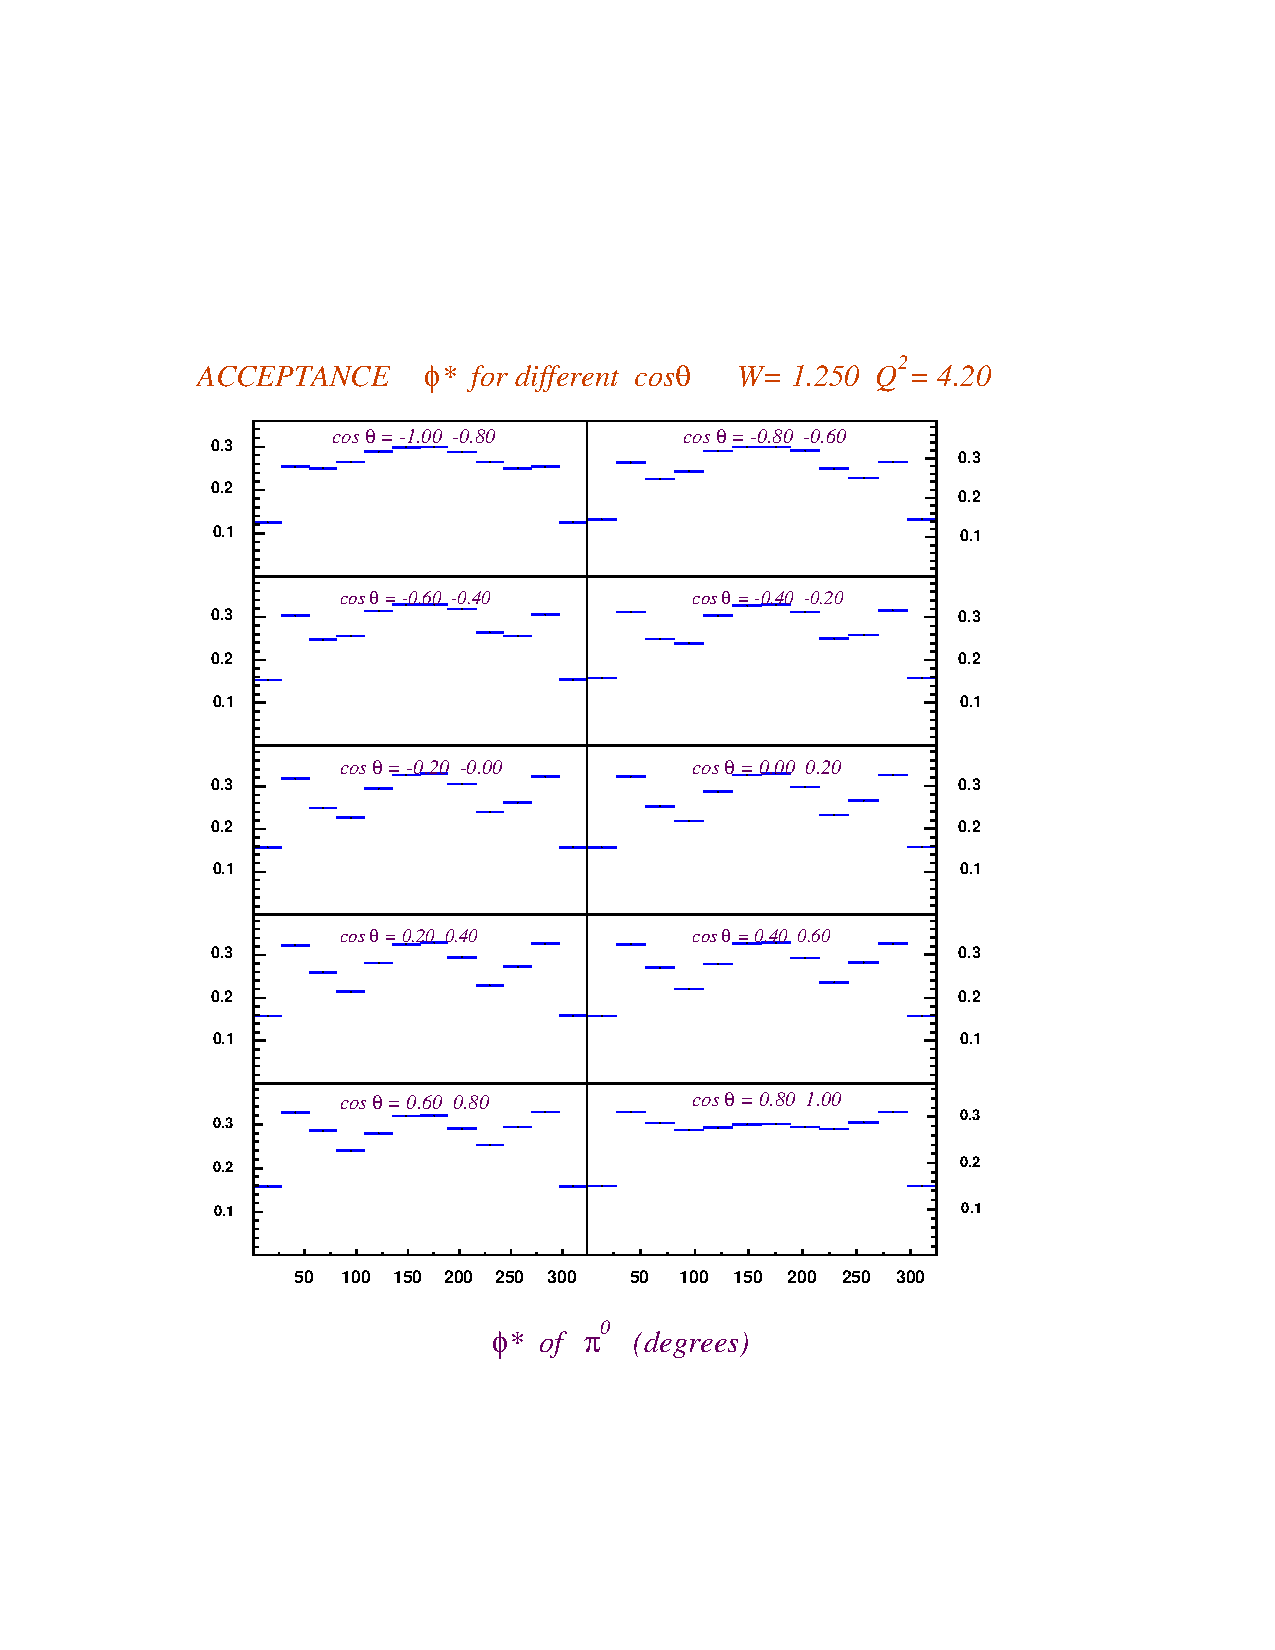
\includegraphics[width = 11cm, bb=140 120 480 600]{acceptance/img/geom_acc} 
%   \caption[]
%           { Geometrical acceptance for a particular $W$m $Q^2$ bin as a function
%                 of $\phi^*$ for different $\cos\theta^*$ bins. The B.H. cut affects
% 		the distributions at $\phi_{\pi^0}^*$ extremes because it drops events with $\phi_P^* \sim 180^0$. }
%  \label{fig:geom_acc}
%  \end{center}
% \end{figure}

